\section{Input Mechanisms}
\label{research:InputMechanisms}
While having an intuitive user interface is crucial for any piece of software, especially when it comes to first impressions and ease of access, I also wanted to focus on the experience of long-term or frequent users — often referred to as power users. These users typically benefit from streamlined workflows that reduce reliance on the mouse or repetitive UI interactions. For them, keyboard shortcuts (or touch gestures on tablets) can significantly increase efficiency, enabling them to complete tasks faster and stay in a focused flow state. By supporting these methods of interaction, software becomes not only accessible to new users but also highly performant for experienced ones.

There's also a cognitive benefit to shortcuts - once committed to muscle memory, they eliminate the need to hunt through menus or click through UI layers. This kind of frictionless interaction turns a tool into something that “disappears” into the background, letting users focus on their ideas rather than the mechanics of using the software. In note-taking and creative tools, where users are often juggling multiple concepts at once, minimizing interaction friction is especially important.

Recognizing this, I started exploring how best to implement shortcut support within my own project. Many software platforms — from word processors to design tools — have already standardized a wide set of keyboard shortcuts that users have come to expect. Commands like Ctrl+C for copy, Ctrl+Z for undo, and Ctrl+S for save are now almost universal across desktop environments. I felt it was important to honour these conventions wherever possible to make my software feel instantly familiar and reduce the learning curve for new users.

To do this effectively, I researched different keyboard mappings used in popular apps like Notion, VSCode, Obsidian, and even design tools like Figma and Adobe Suite. I paid particular attention to how these tools balance common shortcuts with app-specific ones, and how they communicate these to users through tooltips, menus, or shortcut cheat sheets. This gave me a good sense of how to strike a balance between discoverability and depth.

In the end, the goal is to create a tool that scales with its user — accessible enough for beginners, but deep and efficient for those who want to master it. Implementing a thoughtfully designed shortcut system is a small but powerful way of achieving that, and something I plan to continue refining as my app evolves.

\begin{figure}[H]
\centering
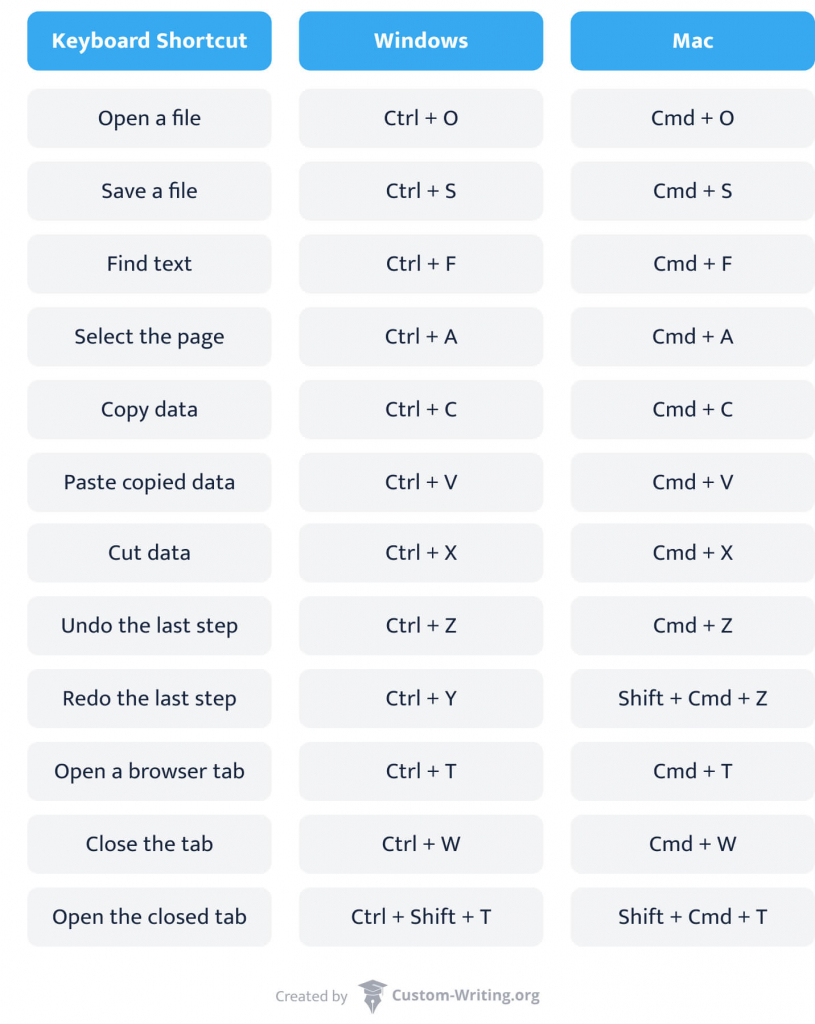
\includegraphics[width=0.6\textwidth]{Research/11_InputMechanisms/media/diagram1.png}
\caption{Example of a keyboard shortcut cheat sheet from CustomWriting.org}
\end{figure}


\begin{figure}[H]
\centering
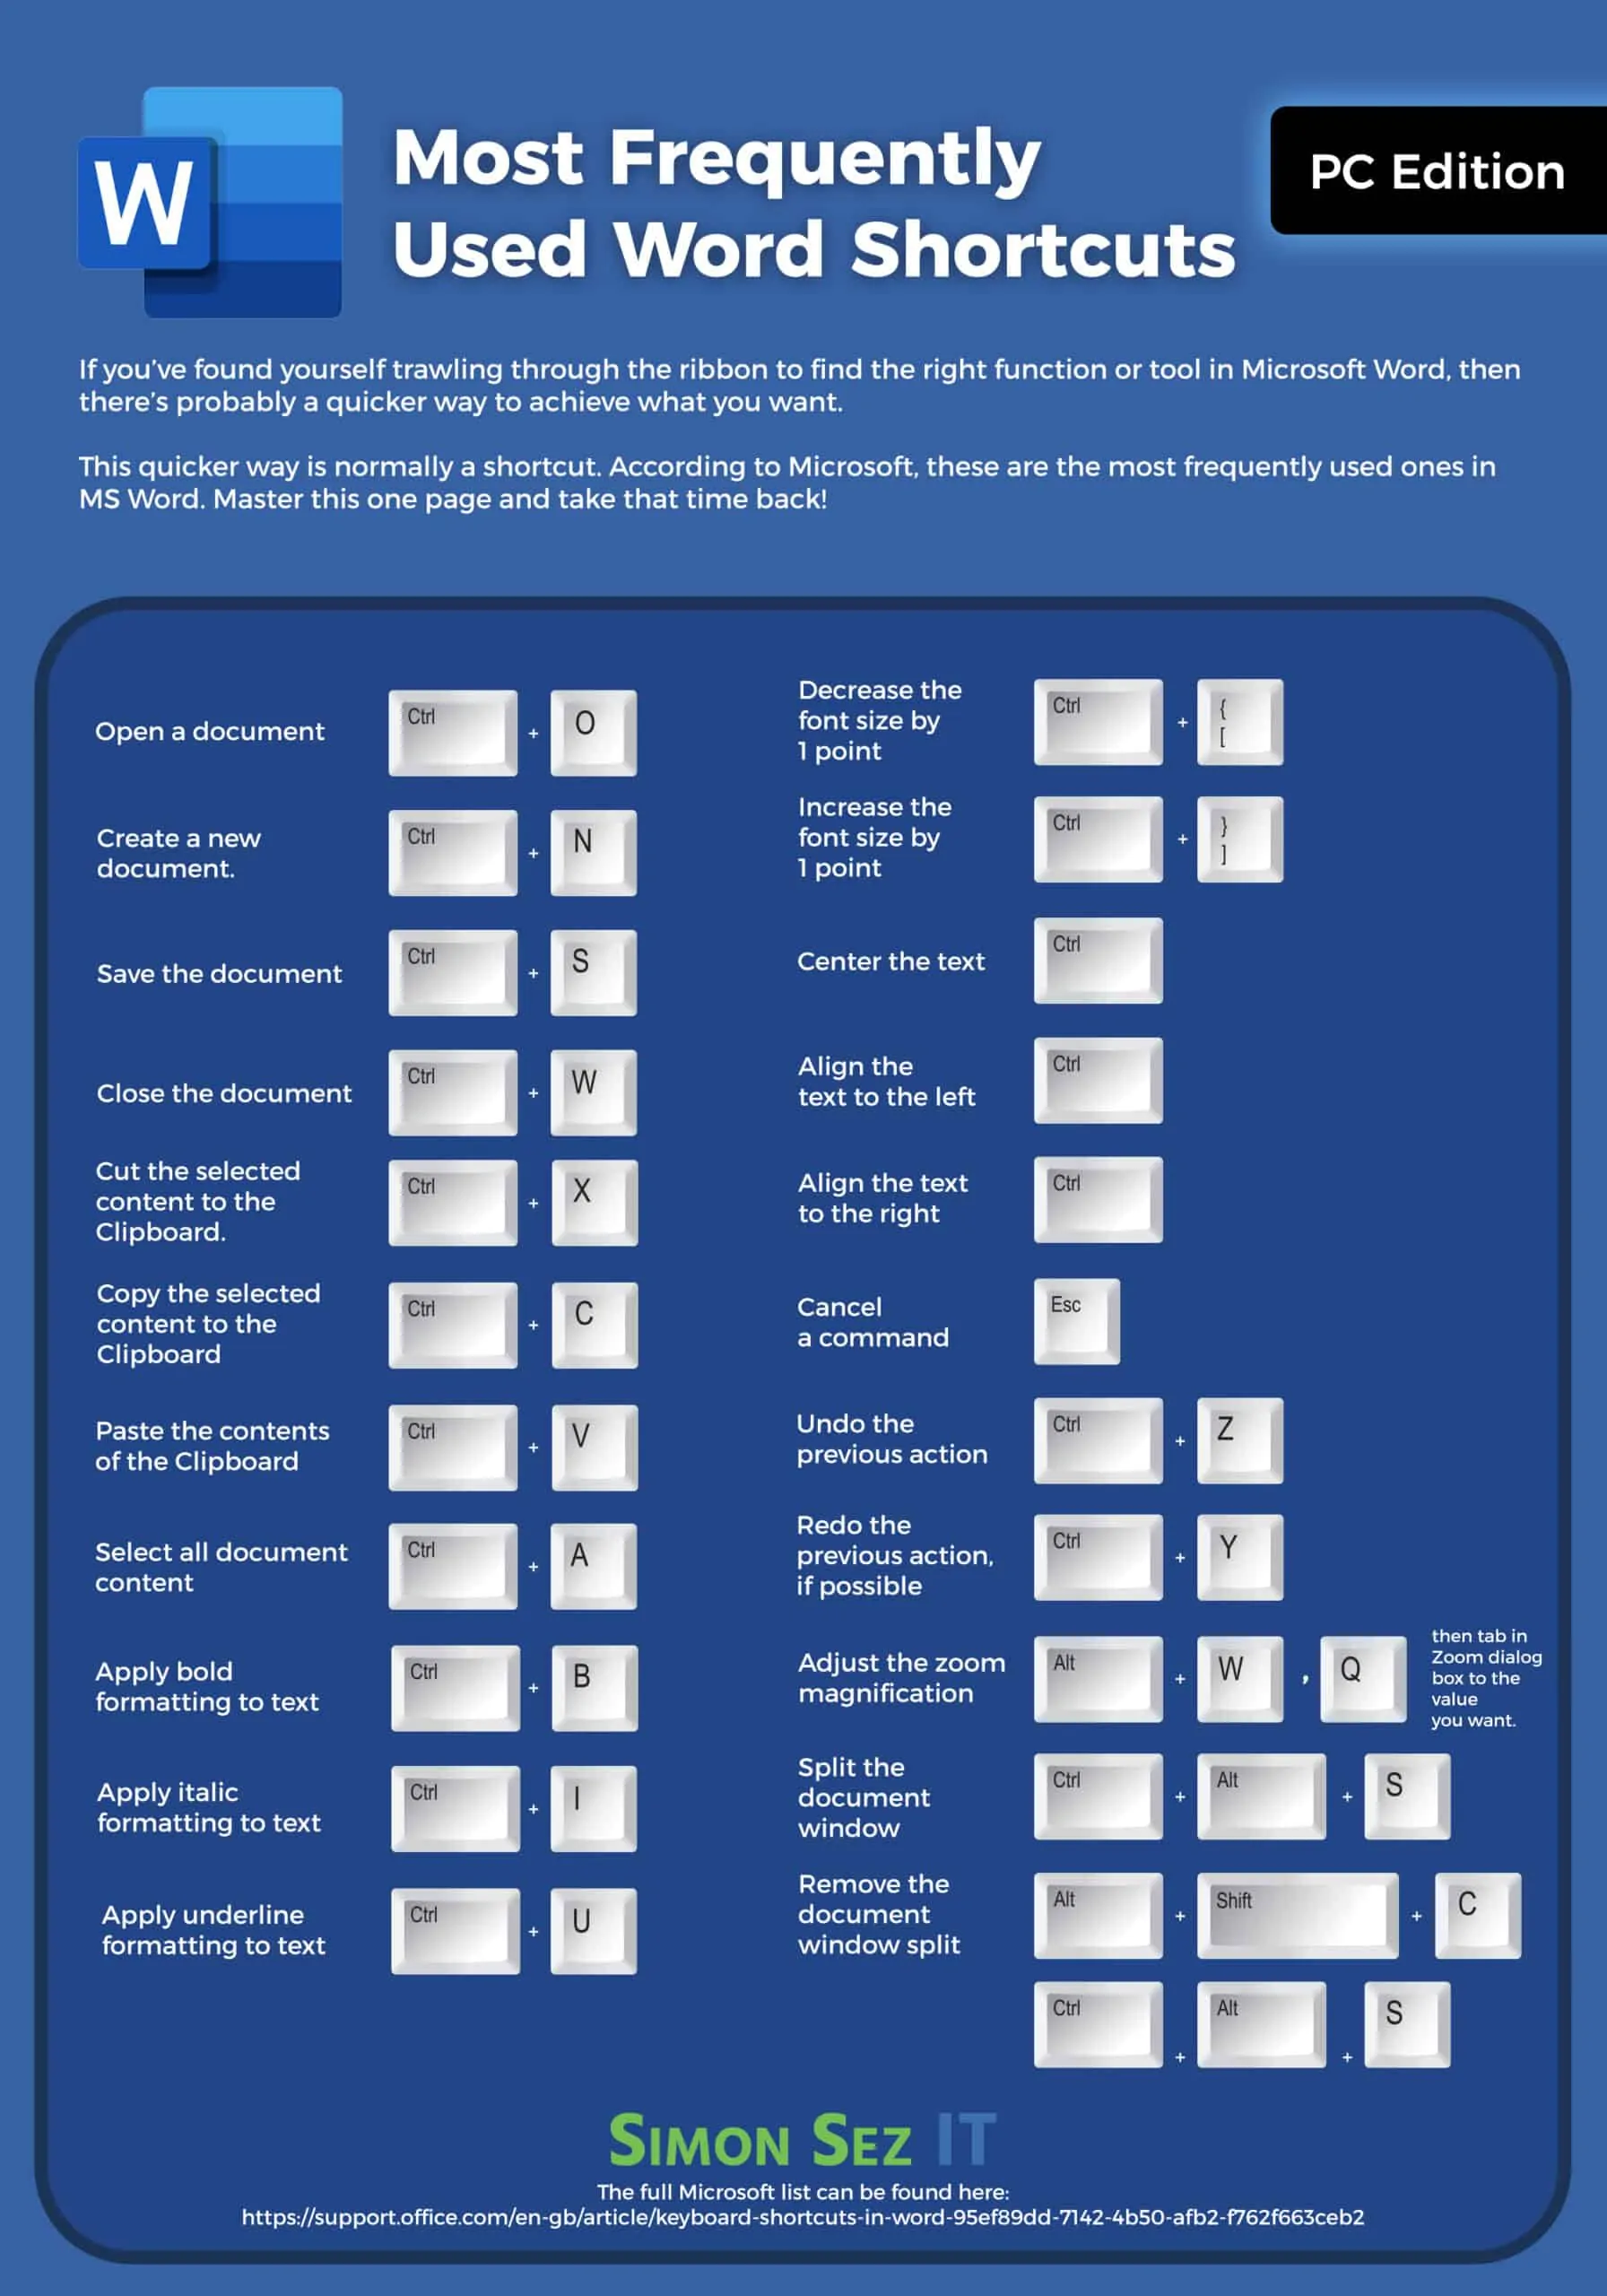
\includegraphics[width=0.6\textwidth]{Research/11_InputMechanisms/media/diagram2.png}
\caption{Thirdy Party keyboard shortcut cheat sheet for word from SimonSezIt}
\end{figure}

\begin{figure}[H]
\centering
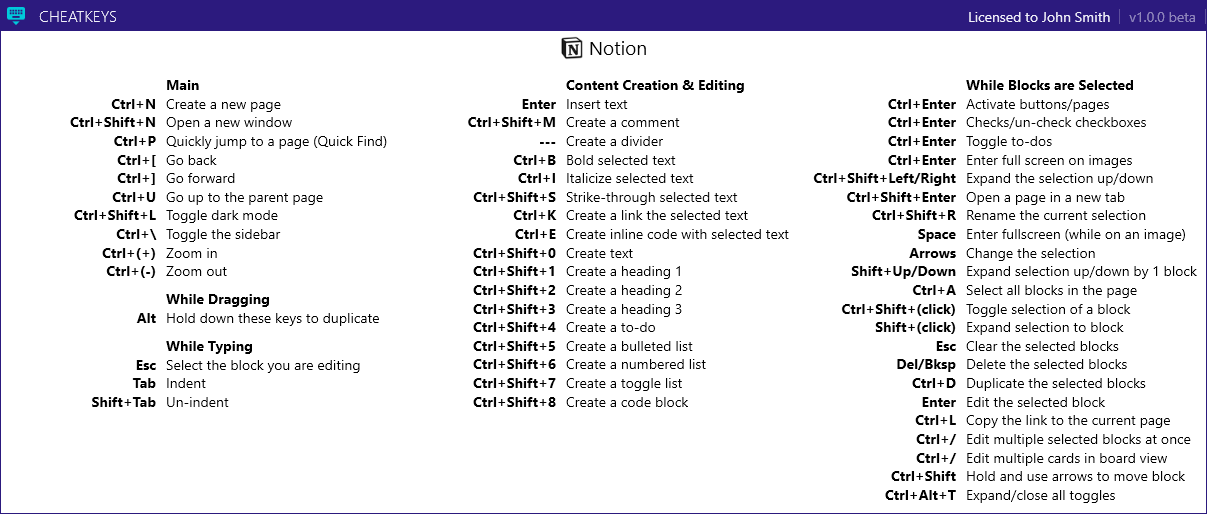
\includegraphics[width=0.6\textwidth]{Research/11_InputMechanisms/media/diagram3.png}
\caption{Example of a keyboard shortcut cheat sheet from Notion}
\end{figure}